\clearpage
\section{Anhang}
\label{sec:appendix}

Im Anhang wird das Vorgehen in den verschiedenen Abschnitten näher erläutert. Es werden alle Hintergrundinformationen, die nicht direkt für die Arbeit selbst relevant sind, gesammelt und dargestellt.

\subsection{Vorgehen bei der Untersuchung der Curricula}\label{sec:analysis_curric}
Um auszuarbeiten, wie die aktuelle Situation an deutschen Hochschulen und Universitäten ist, wurde der Hochschulkompass der Hochschulrektorenkonferenz verwendet \cite{hochschulkompass}.
Auf der Webseite wurden Studiengänge der Informatik gesucht und nach folgenden Kriterien mithilfe der Filterfunktion der Webseite sortiert:

\begin{itemize}
    \item Abschluss Bachelor/Bakkalaureus (Da Programmieranfänger betrachtet werden sollen, ergibt es im Kontext keinen Sinn, weiterführende Studiengänge oder Masterprogramme zu berücksichtigen)
    \item Studientyp Grundständig (Siehe Abschluss Bachelor/Bakkalaureus)
    \item Fachsuche Informatik (Speziellere Studiengänge wie Bioinformatik und Wirtschaftsinformatik wurden ausgeschlossen, um Überschneidungen zwischen den Hochschulen zu meiden. Es wurde immer ein Studiengang pro Institution untersucht, der sich möglichst nah an der Allgemeinen Informatik kategorisieren lässt)
    \item Studienfeld Angewandte Informatik oder Informatik (Siehe Fachsuche)
    \item Studienformen Vollzeitstudium (Ein weiteres Kriterium, um Überschneidungen zu meiden und die Studiengänge weiter auszusortieren)
    \item ohne Lehramt (Wurde in den Filtern aussortiert, da die Lerninhalte sowohl Informatik als auch Erziehungswissenschaften umfassen, und somit nicht im Fokus der Arbeit liegen)
\end{itemize}

Nach der Anwendung der Filter wurden noch insgesamt 425 Treffer angezeigt, die erst im späteren Verlauf der Arbeit weiter reduziert wurden (siehe \nameref{sec:sorting}).

\subsubsection{Zeit Verwaltung}\label{sec:time_management}
Da die Curricula-Analyse nicht der Schwerpunkt der Bachelorarbeit sein sollte, musste entschieden werden, wie viel Zeit in das Thema investiert werden soll.
Hierbei wurden mehrere Risiken gesehen. Zum einen ist es möglich, dass man durch Internetrecherche alleine nicht erschließen kann, welche Inhalte ein Modul hat.
Zum anderen ist das größere Risiko wahrscheinlich der Zeitfaktor. Es ist ungewiss, wie lange es dauert, jedes Modul zu untersuchen, da jede Institution ihre Informationen anders sortiert, bereitstellt und handhabt.

Um die Zeit in einem realistischen Rahmen zu halten, wurde in Erwägung gezogen, einen Zeitraum festzulegen, in dem so viele Studiengänge wie möglich betrachtet werden, und diese anschließend die Forschungsmenge darstellen. Dieser Zeitraum könnte etwa auf 2 Arbeitstage fallen. Auch wurde abgewägt, die Studiengänge nach Anzahl der Studierenden zu sortieren und die 50 am besten besuchten Institutionen zu betrachten.

Es wurde allerdings ebenfalls notiert, dass das unsicherste Kriterium hier die Zeit war, die benötigt wird, um einen Studiengang zu untersuchen. Möglicherweise müssen die Methoden zur Reduktion der Zeit gar nicht angewandt werden, wenn sich die Risiken nicht erfüllen. Zunächst wurde daher versucht, abzuwägen, wie lange Analysezeit grob einzuschätzen war.
In einer isolierten Probe wurden fünf zufällige Universitäten betrachtet (In diesem Fall die ersten fünf Suchergebnisse des Hochschulkompasses, die HS Furtwangen, die Ruhruniversität Bochum, die Hochschule Fulda, die Friedrich-Schiller-Universität Jena, und die Hochschule Konstanz).
Es dauerte etwa 10 Minuten, um entsprechende Informationen über alle 5 Studiengänge zu erlangen.
Bei den 121 verbleibenden Informatik-Studiengängen wurde die Zeitdauer also grob auf 4 Stunden eingeschätzt, ein realistischer Zeitraum zur Sammlung der Daten. Mit diesen neuen Informationen wurden die Methoden zur Zeitreduktion wieder verworfen.

Letztendlich wurde für die Analyse doch ein ganzer Arbeitstag benötigt, aber die reduzierte Menge der Studiengänge durch die Filter war bereits genügend, um die Daten in einem angemessenen Zeitraum zu sammeln.

\subsubsection{Untersuchung der Daten}\label{sec:sorting}
Bei der Analyse der Curricula wurde systematisch vorgegangen. Mithilfe eines Webscrapers wurden alle nötigen Informationen als JSON extrahiert und in einer Excel-Tabelle sortiert.
Es wurde festgestellt, dass die Filterfunktion des Hochschulkompasses nicht ausreichend war, um die Datenmenge zu reduzieren. Die Studiengänge wurden daher noch einmal manuell aussortiert, nach weiteren Kriterien.
Ein Studiengang wurde demnach aussortiert, wenn eines der folgenden Kriterien zutraf.

\begin{itemize}
    \item Kein allgemeiner Informatikstudiengang (Zum Beispiel Bioinformatik oder Wirtschaftsinformatik)
    \item Zweitfach oder Nebenfach Informatik
    \item Teilzeitstudium
    \item Mehrere Studienorte für einen Studiengang (Hierbei sind die angebotenen Module teils nicht eindeutig zuordenbar)
    \item Doppelte Studiengänge für eine Institution (Etwa wenn sowohl Angewandte als auch Allgemeine Informatik angeboten wird. Es wurde immer der allgemeinere Studiengang gewählt. Zwischen internationalen und deutschen Studiengängen wurde immer der deutsche Studiengang gewählt)
\end{itemize}

Für die meisten Studiengänge ließen sich die nötigen Informationen in sehr kurzen Zeiträumen mit einer Suche nach dem Studienverlaufsplan, sowie dem Modulhandbuch für die Informatik finden.
Hierbei wurde der Studienverlaufsplan genutzt, um herauszufinden, welcher Kurs als Einführung in die Programmierung im ersten Semester dient, und das Modulhandbuch, um zu extrahieren, welche Programmierparadigmen und Sprachen im Kurs verwendet werden.

\paragraph{Unterschied der Datensätze Unspezifisch und Keine Infos}\label{sec:unspecified_vs_na}
Nicht alle Module listeten die benötigten Informationen. Es wird in der Analyse grundsätzlich unterschieden zwischen zwei Fällen. Zum einen, Studiengänge, die zwar ein Modulhandbuch zur Verfügung stellten, dieses aber nicht explizit spezifiziert, welche Paradigmen und Programmiersprachen verwendet werden (Markiert als "Unspezifisch"). Zum anderen gibt es noch den Fall, dass kein Modulhandbuch öffentlich zur Verfügung steht. Dies kann etwa der Fall sein, wenn die Institution Informationen nur auf Anfrage herausgibt, oder das Modulhandbuch einfach nicht aufzufinden war. Es wurde davon abgesehen, die Institutionen zu kontaktieren, um einen neuen ungewissen Faktor in der Arbeit zu vermeiden. Die Studiengänge ohne Modulhandbuch wurden leer gelassen und sind in der Excel-Tabelle rot markiert. In der Grafik zur Darstellung der Ergebnisse sind diese Datensätze in "Keine Infos" kategorisiert.
\\
Die Excel-Tabelle mit den extrahierten Daten lässt sich im Repository der Bachelorarbeit finden \cite{repoxlsx}.

\subsection{Ähnliche Forschungsergebnisse zum Forschungsteil}\label{sec:similar_srcs}
Da zum Zusammenhang von CT, Lerntypen und Programmierparadigmen wenig vorhandene Quellen gefunden wurden, basieren viele Annahmen des Forschungsteils auf Spekulationen, die auf Basis des Rechercheteils gemacht wurden.
Um genauere Forschungsergebnisse zu erzielen, würde es sich anbieten, eine eigene Studie im Rahmen der Bachelorarbeit durchzuführen. Dies konnte in dieser Arbeit aufgrund von zeitlichen Einschränkungen nicht umgesetzt werden, wäre allerdings eine mögliche Erweiterung der Forschungsfragen.

Die Quelle zum Thema CT und Lerntypen \cite{chen} bestätigte vorhandene Forschungsergebnisse nachträglich und erweiterte diese leicht. Es gibt auch andere Quellen, die allerdings nicht komplett mit den betrachteten Themen übereinstimmen. Hierzu wurden mehrere Untersuchungen von CT gefunden, allerdings nicht speziell im Kontext von Programmierparadigmen und Lerntypen.

Beispielweise wurde hierbei vor der Verfassung des Forschungsteils eine Arbeit speziell zum Thema Entwicklung von CT mit Lernstilen betrachtet \cite{boardgames}, allerdings verwendete die Arbeit das Lerntypenmodell nach David Kolb. Die Arbeit analysierte zudem eher die Methodiken, die verwendet werden können, um CT Kompetenzen möglichst effizient zu lehren, und bietet weniger Inhalt hinsichtlich des Zusammenhanges mit einzelnen Lerntypen.

Eine weitere Quelle \cite{michaelson} zum Thema Programmierparadigmen und CT half, die Wahl der häufigsten Paradigmen im Rechercheteil zu bestätigen. Allerdings stellt diese Arbeit eher fest, dass CT eigentlich ein eigenes Paradigma der Programmierung ist und als solches angesehen werden sollte. Weniger wird CT in den Kontext von anderen Programmierparadigmen wie OO Programmierung, Prozedurale Programmierung und weitere gesetzt. Von daher konnten die Schlussfolgerungen der Arbeit eher schwierig für den Forschungsteil verwendet werden.

\subsection{Auswahl des Problems für den Selbstversuch}\label{sec:choice_prac}
Die Auswahl des Programmierproblems in Abschnitt 4 der Arbeit erfolgte an mehreren Kriterien. Es sollte ein relativ einfaches Problem gewählt werden, das eher einen Zweck demonstriert als kreative Lösungen erfordert.
Zunächst wurde hierbei entschieden, einen Algorithmus zur automatischen Lösung und Erstellung eines Sudoku zu schreiben.
Bei einem Sudoku handelt es sich um ein klassisches Rätsel, bei dem auf einem 9x9 großen Feld in jeder Zeile, Spalte, und in jeder 3x3 großen Box jede Zahl von 1 bis 9 nur ein mal vorkommen darf.

Das Problem eignete sich zum Untersuchen und Lernen von funktionaler Programmierung (FP), da alle wichtigsten Aspekte von FP benötigt wurden, um das Problem im Paradigma erfolgreich umzusetzen (Rekursion, Funktionen höherer Ordnung, Komposition, Unveränderlichkeit). Es wurden ebenfalls alle CT Aspekte ausreichend abgedeckt.

\begin{description}
    \item[Dekomposition] Herunterbrechen in Teilprobleme. Beispielsweise Validierung des Sudoku, dann Untersuchen der Spalten, Zeilen und Boxen separat.
    \item[Abstraktion] Rätsel in Datenstrukturen umwandeln. Beispielsweise Überlegungen, wie das Brett und die Felder am besten im Code abgebildet werden können.
    \item[Algorithmen] Zur Implementierung des Solvers.
    \item[Debugging] Wie kann das Sudoku effizient gelöst werden? Evaluierung der Lösung und Erkennen von Fehlerpotenzial in den einzelnen Unterfunktionen.
\end{description}

Letztendlich wurde allerdings doch ein anderes Problem gewählt, da Sorgen hinsichtlich der Umsetzbarkeit im gegebenen Zeitrahmen bestanden.
Es wurde letztendlich die Türme von Hanoi als Aufgabe für den Selbstversuch entschieden. Dies geschah hauptsächlich aus zwei Gründen. Zum einen gab es eine persönliche Empfehlung des betreuenden Prüfers. Zum anderen wurde das Problem im ersten Aufgebenblatt des verwendeten Kurses betrachtet, um Haskell zu lernen. Das Vorhandensein der Türme von Hanoi in einem Anfängerkurs für FP vermittelte den Eindruck, dass die Aufgabe besonders geeignet sein könnte, um den Einstieg in die FP zu simulieren.
Das Problem vertritt ebenfalls wichtige Aspekte von FP, vor allem das Konzept des Backtrackings. Auch die CT Aspekte waren wiederum erkennbar vertreten, was letztendlich zur Entscheidung führte.

\begin{description}
    \item[Dekomposition] Überlegung, welche Teilprobleme es gibt. Ein bisschen weniger offensichtlich als beim Sudoku Solver, aber beispielsweise die Validierung der Züge und die tatsächliche Durchführung sind zwei verschiedene Verantwortungen.
    \item[Abstraktion] Überlegung, wie die Pins und Holzplatten abgebildet werden können. Wie wird deutlich, welche Platte zu welchem Pin gehört? Wie wird die Größe der Platten deutlich? Hierbei können beispielsweise Integer verwendet werden.
    \item[Algorithmen] Zur tatsächlichen Implementierung des Problems.
    \item[Debugging] Ebenso wie der Sudoku Solver gibt es hier mehrere Lösungen, die abgewägt werden können.
\end{description}

\subsection{Vorgehen im Selbstversuch}\label{sec:tools_prac}
Der Autor hatte vor der Bachelorarbeit keinerlei Vorkenntnisse in FP und Haskell. Um die Sprache zu lernen, wurde den offiziellen Empfehlungen der Haskell-Dokumentation gefolgt. Hierbei war das sogenannte read-eval-print-loop (REPL) besonders hilfreich. Die interaktive Programmierumgebung nimmt einzelne Nutzerinputs, evaluiert diese und gibt den Output an den Nutzer zurück. Im Kontext der CIS 194 Vorlesung wurde das REPL ebenfalls zur Einführung in Haskell-Variablen verwendet.
Personen ohne Vorkenntnisse können so schnell und barrierefrei mit der Syntax und den Ausdrücken in Haskell experimentieren und so praktische, erste Programmiererfahrungen machen.
Die Arbeit mit der REPL begünstigt zudem durch die extrem schnelle Feedbackschleife eine aktivere Arbeitsweise, die ein schnelles Testen und Fehlschlagen ermöglicht.

\begin{figure}[H]
    \centering
    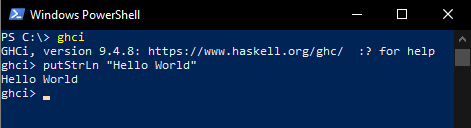
\includegraphics[width=1\linewidth]{Figures/Anhang/ghci}
    \caption{Verwendung von GHCi in der Windows PowerShell}
\end{figure}

Um Haskell Syntax und generelle Prinzipien zu lernen, wurden zunächst die ersten Aufgaben der CIS 194 Hausaufgaben bearbeitet.